\section{Graphs}
Suppose \(\Gamma\) contains \((m-1)K_2\) as a subgraph i.e. \(\Gamma\) contains \(m-1\) disjoint edges.
Then, \(\Gamma\) has at least \((m-1)V(K_2) = 2m - 2\) vertices.

\begin{lem}
    If \(\Gamma - \Lambda\) is \(K_{1,3}\)
    for any subgraph \(\Lambda\) isomorphic to \((m-1)K_2\),
    then \(\Gamma\) is \(K_{m, m+2}\) for some \(m \ge 1\).
\end{lem}

\begin{proof}
    First notice that \(V(\Gamma) - V(\Lambda) = V(K_{1,3})\) implies that \(V(\Gamma) = 2m + 2\).

    We claim that \(\Gamma\) cannot contain any odd cycles.
    To see this, suppose the vertices \(\{u_i\}_{i=1}^n\) form an \(n\)-cycle in \(\Gamma\) for some odd \(n \ge 3\).


    If \(\Gamma - \{u_i\}_{i=1}^n\) contains \((m-1)K_2\) as a subgraph,
    then \(V(\Gamma - \{u_i\}_{i=1}^n - (m-1)K_2) = V(K_{1,3})\).
    However, this means \(2m + 2 - n - 2(m-1) = 4\) implying \(n = 0\), a contradiction.
    So, suppose \(\Gamma - \{u_i\}_{i=1}^n\) does not contain \((m-1)K_2\) as a subgraph,
    then \(\Lambda\) contains at least two of the vertices in \(\{u_i\}_{i=1}^n\).

    % This is fine since if there are k edges in the cycle we can just choose the first 2k vertices
    Without a loss of generality suppose \(\{u_i\}_{i=1}^{2k}\) belong to \(\Lambda\)
    for some \(k \ge 1\). 
    Since \(n\) is odd, at least one of the vertices in the cycle, say \(u_{2k+1}\) must belong to \(\Gamma - \Lambda\).

    We proceed by cases on the valence of \(u_{2k+1}\) in \(\Gamma - \Lambda\).

    %TODO fix these cases
    % diagram could look like:
    % | | ... |    | \ | \ | \ ... |     Y
    %   m-1-k       k edges in cycle    K_1,3

    \textbf{Case 1:} \(u_{2k+1}\) has valence \(1\) in \(\Gamma - \Lambda\).
    Let \(u_4\) and \(u_5\) be the other valence \(1\) vertices in \(\Gamma - \Lambda\)
    and \(u_6\) be the valence \(3\) vertex in \(\Gamma - (m-1)K_2\).

    \begin{figure}[h!]
    \centering
    \begin{tikzpicture}
        \node (v1) at (0,1) {};
        \node (w1) at (0,3) {};
        \node (vmm1) at (1,1) {};
        \node (wmm1) at (1,3) {};
        \draw (v1) -- (w1);
        \draw (vmm1) -- (wmm1);

        \node (u1) at (2, 3) {\(u_1\)};
        \node (u2) at (2, 1) {\(u_2\)};
        \node (u3) at (3, 2) {\(u_3\)};

        \draw (u1) -- (u2);
        \draw (u2) -- (u3);
        \draw (u3) -- (u1);

        \node (u4) at (3, 1) {\(u_4\)};
        \node (u5) at (3, 0) {\(u_5\)};

        \node (u6) at (4, 1) {\(u_6\)};

        \draw (u6) -- (u3);
        \draw (u6) -- (u4);
        \draw (u6) -- (u5);
    \end{tikzpicture}
    \end{figure}

    Immediately we see a contradiction arise as \(\Gamma - \{u_1, u_2, u_3\}\) contains \((m-1)K_2\) as a subgraph.

    \textbf{Case 2:} \(u_3\) has valence \(3\) in \(\Gamma - (m-1)K_2\).
    Let \(u_4\), \(u_5\), and \(u_6\) be the other valence \(1\) vertices in \(\Gamma - (m-1)K_2\).

    \begin{figure}[h!]
    \centering
    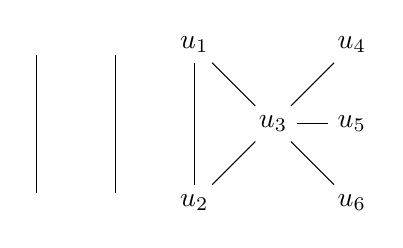
\begin{tikzpicture}
        \node (v1) at (0,0) {};
        \node (w1) at (0,2) {};
        \node (vmm1) at (1,0) {};
        \node (wmm1) at (1,2) {};
        \draw (v1) -- (w1);
        \draw (vmm1) -- (wmm1);

        \node (u1) at (2, 2) {\(u_1\)};
        \node (u2) at (2, 0) {\(u_2\)};
        \node (u3) at (3, 1) {\(u_3\)};

        \draw (u1) -- (u2);
        \draw (u2) -- (u3);
        \draw (u3) -- (u1);

        \node (u4) at (4, 2) {\(u_4\)};
        \node (u5) at (4, 1) {\(u_5\)};
        \node (u6) at (4, 0) {\(u_6\)};

        \draw (u3) -- (u4);
        \draw (u3) -- (u5);
        \draw (u3) -- (u6);
    \end{tikzpicture}
    \end{figure}

    Erasing the \(m-2\) edges to the left in the figure above along with the edge \(u_2 u_3\), we must have the following
    edges for the resulting subgraph to be \(K_{1,3}\).

    \begin{figure}[h!]
    \centering
    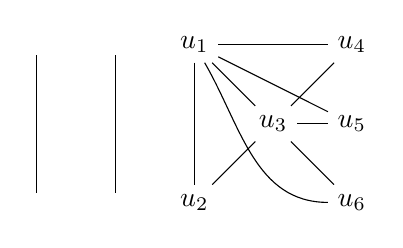
\begin{tikzpicture}
        \node (v1) at (0,0) {};
        \node (w1) at (0,2) {};
        \node (vmm1) at (1,0) {};
        \node (wmm1) at (1,2) {};
        \draw (v1) -- (w1);
        \draw (vmm1) -- (wmm1);

        \node (u1) at (2, 2) {\(u_1\)};
        \node (u2) at (2, 0) {\(u_2\)};
        \node (u3) at (3, 1) {\(u_3\)};

        \draw (u1) -- (u2);
        \draw (u2) -- (u3);
        \draw (u3) -- (u1);

        \node (u4) at (4, 2) {\(u_4\)};
        \node (u5) at (4, 1) {\(u_5\)};
        \node (u6) at (4, 0) {\(u_6\)};

        \draw (u3) -- (u4);
        \draw (u3) -- (u5);
        \draw (u3) -- (u6);

        \draw (u1) -- (u4);
        \draw (u1) -- (u5);
        \draw (u1) to [out=-60, in=180] (u6);
    \end{tikzpicture}
    \end{figure}

    Similarly, by erasing the \(m-2\) edges to the left along with the edge \(u_1 u_3\), we must have the following.

    \begin{figure}[h!]
    \centering
    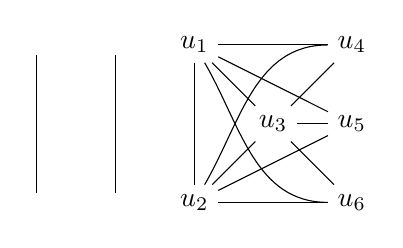
\begin{tikzpicture}
        \node (v1) at (0,0) {};
        \node (w1) at (0,2) {};
        \node (vmm1) at (1,0) {};
        \node (wmm1) at (1,2) {};
        \draw (v1) -- (w1);
        \draw (vmm1) -- (wmm1);

        \node (u1) at (2, 2) {\(u_1\)};
        \node (u2) at (2, 0) {\(u_2\)};
        \node (u3) at (3, 1) {\(u_3\)};

        \draw (u1) -- (u2);
        \draw (u2) -- (u3);
        \draw (u3) -- (u1);

        \node (u4) at (4, 2) {\(u_4\)};
        \node (u5) at (4, 1) {\(u_5\)};
        \node (u6) at (4, 0) {\(u_6\)};

        \draw (u3) -- (u4);
        \draw (u3) -- (u5);
        \draw (u3) -- (u6);

        \draw (u1) -- (u4);
        \draw (u1) -- (u5);
        \draw (u1) to [out=-60, in=180] (u6);

        \draw (u2) to [out=60, in=180] (u4);
        \draw (u2) -- (u5);
        \draw (u2) -- (u6);
    \end{tikzpicture}
    \end{figure}

    Erasing the \(m-2\) edges to the left along with the edge \(u_1 u_4\) results in a subgraph with a \(3\)-cycle,
    contradicting that \(\Gamma - (m-1)K_2\) is always \(K_{1,3}\).

    Thus, \(\Gamma\) does not contain any \(3\)-cycles.
    We claim that \(\Gamma\) does not contain any other odd cycles.
    To see this, suppose \(\Gamma\) contains an odd cycle \(C\) with more than \(3\) vertices.



    We claim that \(\Gamma\) is complete bipartite.
    To see this, suppose there exist vertices \(x\) and \(y\) in different partite sets of \(\Gamma\)
    such that there is no edge between \(x\) and \(y\).
    Since \(\Gamma\) contains \((m-1)K_2\) as a subgraph,
    \(x\) and \(y\) do not belong to this subgraph.
    However, \(\Gamma - (m-1)K_2\) must contain \(x\) and \(y\)
    yet \(K_{1,3}\) is connected.

    Finally, to see that \(\Gamma\) is \(K_{m, m+2}\),
    let \(A\) and \(B\) be the partite sets of \(\Gamma\).
    Since the subgraph \((m-1)K_2\) contains \(m-1\) vertices from \(A\) and \(m-1\) vertices from \(B\),
    it follows that \(A\) contains \(1\) vertex in \(\Gamma - (m-1)K_2\) and \(B\) contains \(3\) vertices.
    Hence \(\abs{A} = m\) and \(\abs{B} = m + 2\).

\end{proof}

\begin{lem}
If \(\Gamma - (m-1)K_2\) is always \(K_3\), then \(\Gamma\) is \(K_{2m+1}\).
\end{lem}

\begin{proof}

\end{proof}

\begin{lem}
If \(\Gamma - (m-1)K_2\) is always the cycle graph \(C_4\), then \(\Gamma\) is \(K_{m+1, m+1}\).
\end{lem}

\begin{proof}

\end{proof}